\documentclass[final]{beamer}

\newcommand{\trucPleinEcran}[1]{{%
  \setbeamertemplate{navigation symbols}{}%
  \setbeamertemplate{background}{}%
  \setbeamertemplate{background canvas}{%
    #1
   }%
   \frame[plain]{}%
}}

\newcommand{\figurePleinEcran}[1]{{%
  \setbeamertemplate{navigation symbols}{}%
  \setbeamertemplate{background}{}%
  \setbeamertemplate{background canvas}{%
    \hfill%
    \includegraphics[width=\paperwidth,height=\paperheight,keepaspectratio]{#1}%
    \hfill%
   }%
   \frame[plain]{}%
}}

%\usepackage{pgfpages}
%\pgfpagesuselayout{2 on 1}[a4paper,border shrink=5mm]

\usepackage{amssymb,amsmath}
\usepackage{mathpartir}
\usepackage{xcolor}
\usepackage{wrapfig}
\usepackage{tikz}
\usetikzlibrary{shapes,arrows}
\usetikzlibrary{fit}					% fitting shapes to coordinates
\usetikzlibrary{backgrounds}	% drawing the background after the foreground
%\usepackage[]{graphicx}
%\usepackage[french,noend]{algorithm2e}
\tikzstyle{background}=[rectangle, fill=gray!10, inner sep=0.2cm, rounded corners=5mm]
\tikzstyle{pass}=[shade, shading=axis, rounded rectangle, draw, fill=black!10,
        inner sep=5pt, text width=2cm,
        text badly centered, minimum height=1.2cm,
        font=\bfseries\scriptsize\sffamily]
\tikzstyle{tool}=[rectangle, draw, thick, fill=black!10, inner sep=5pt, text
        width=1.5cm,
        text badly centered, minimum height=.8cm,
        font=\bfseries\scriptsize\sffamily] 

\usepackage{stmaryrd}
\usepackage{fontspec}
\usepackage{xunicode}
\usepackage{xltxtra}
\defaultfontfeatures{Mapping=tex-text}
\setsansfont{Museo Sans}
\setromanfont{Museo}
\setmonofont[Scale=.88]{DejaVu Sans Mono}

\mode<presentation> {
  \usetheme{Singapore}
  \setbeamercovered{transparent}
  \AtBeginSection[]{
    \begin{frame}<beamer| handout>[shrink]
      \frametitle{Plan}
      \tableofcontents[sectionstyle=show/shaded,subsectionstyle=show/shaded/hide]
      %\tableofcontents[sectionstyle=show/show,subsectionstyle=show/show/hide]
    \end{frame}}
  \AtBeginSubsection[]{
    \begin{frame}<beamer| handout>[shrink]
      \frametitle{Plan}
      %\tableofcontents[sectionstyle=show/shaded,subsectionstyle=show/shaded/hide]
      \tableofcontents[sectionstyle=show/shaded,subsectionstyle=show/shaded/hide]
    \end{frame}}
}
%\setbeamertemplate{navigation symbols}{}

\title{\textsc{Traduction d'OCaml vers une variante de Système F}}
\author{Jonathan Protzenko\\sous la direction de François Pottier}
\date{\today}

\begin{document}

\begin{frame}
  \titlepage
\end{frame}

\section{Introduction}

\subsection{Aperçu du problème}

\begin{frame}{Pourquoi traduire?}
  \begin{columns}
    \column{.5\columnwidth}
      \begin{itemize}
        \item On veut augmenter la confiance dans la chaîne de compilation
        \item ``Well-typed programs can't go wrong'' (Milner)
        \item Le système de types d'OCaml est trop complexe
      \end{itemize}
    \column{.5\columnwidth}
      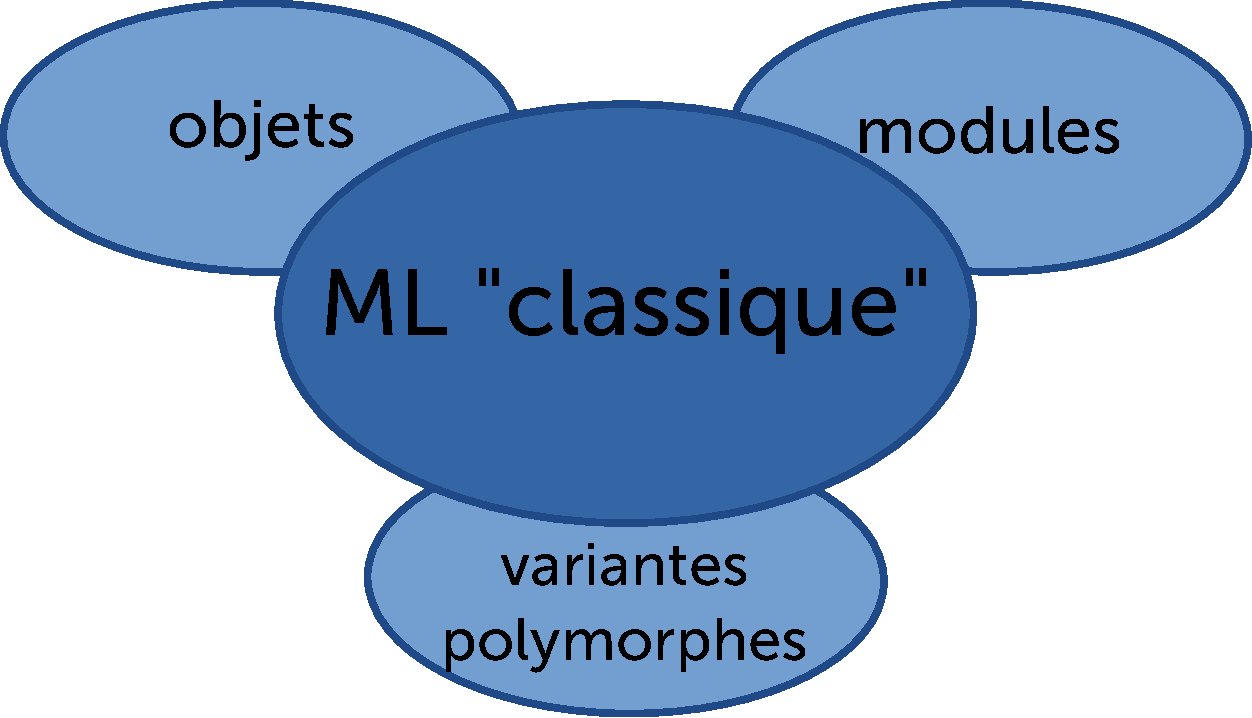
\includegraphics[width=\columnwidth]{ocaml.pdf}
  \end{columns}
  \begin{itemize}
    \item Traduire le programme dans un langage de base
    \item Vérifier le typage \emph{a posteriori}
  \end{itemize}
\end{frame}

\begin{frame}{Objectifs à long terme}
  \begin{itemize}
    \item Fournir un langage intermédiaire pour \emph{effectuer des analyses} et
      compiler plus en avant: expressions \emph{simples}, informations de type
      \emph{riches}.
    \item Augmenter la confiance dans la chaîne de compilation: à défaut de
      prouver la correction du typeur, prouver la cohérence de ses résultats.
    \item Clarifier la sémantique du langage original: quelles sont les
      constructions qui s'expriment bien dans FE+?
  \end{itemize}
\end{frame}

\begin{frame}{Dans les grandes lignes…}
  \begin{center}
    \begin{tikzpicture}
      [node distance = 1cm, auto, every node/.style={node distance=3cm}]
      % Place nodes
      \node [pass] (solve) {Résolution de contraintes};
      \node [left of=solve, node distance=3.5cm] (phantom) {};
      \node [pass, above of=phantom, node distance=1cm] (gen) {Génération de contraintes};
      \node [pass, dashed, below of=phantom, node distance=1cm] (gen2) {Autre langage de surface};
      \node [pass, right of=solve, node distance=3.5cm] (camlx) {AST annoté (CamlX)};
      \node [pass, below of=camlx] (fe) {Langage Core (Système FE+)};
      \node [tool, left of=fe] (typecheck) {Type-checking};
      %\node [block, below of=solve] (unify) {Moteur d'unification};
      % Draw edges
      \draw [->, thick] (gen) -- (solve);
      \draw [->, thick, dashed] (gen2) -- (solve);
      \draw [->, thick] (solve) -- (camlx);
      \draw [->, thick] (camlx) -- (fe);
      \draw [->, thick] (typecheck) -- (fe);
      %\path [line, <->] (unify) -- (solve);
      \begin{pgfonlayer}{background}
        \node [background, fit=(gen) (gen2) (solve), pin=-100:Inférence] {};
        \node [background, fit=(camlx) (fe), pin=80:Traduction] {};
      \end{pgfonlayer}

    \end{tikzpicture}
  \end{center}
  \footnotesize Le processus se découpe en deux parties~: génération/résolution de
  contraintes, et traductions jusqu'à Système FE+.
\end{frame}

\subsection{Contributions}

\begin{frame}{Trois grands axes de travail}
  \begin{columns}
    \column{.5\columnwidth}
      \begin{itemize}
        \item Récrire un système d'inférence par contraintes (générateur de
          contraintes \emph{et} solveur), et l'adapter pour
          donner un \emph{AST annoté}.
        \item Élaborer un processus de traduction d'un fragment d'OCaml vers un
          langage minimaliste
        \item Concevoir le système de types qui permet de justifier le comportement
          d'OCaml
      \end{itemize}
    \column{.5\columnwidth}
      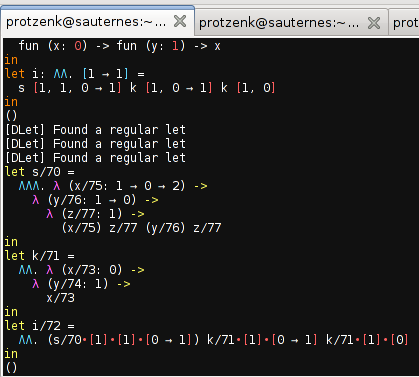
\includegraphics[width=\columnwidth]{screen1.png}
  \end{columns}
\end{frame}

\begin{frame}{Trois langages}

  Les langages suivants sont utilisés:
  \begin{itemize}
    \item CamlX <<~à trous~>> (OCaml annoté)
    \item CamlX <<~tout court~>> (OCaml annoté en De Bruijn)
    \item Système FE+
  \end{itemize}

  Système FE+ est Système $F_\eta$ augmenté avec des coercions explicites, des
  expressions supplémentaires (tuples), des patterns\dots
\end{frame}

\section{Décoration d'ASTs}

\subsection{Le cœur du problème}

\begin{frame}{L'inférence par contraintes}
  \begin{itemize}
    \item Présentation revue d'un algorithme <<~classique~>> (Pottier, Rémy, 2005)
    \item Séparation claire et élégante entre génération et résolution
    \item Préférable à l'implémentation OCaml, performante mais difficile
      d'accès
  \end{itemize}
  Exemple: $$
  \llbracket \lambda z.t : T \rrbracket \quad = \quad
  \exists X_1 X_2.\left(\text{let }z: X_1 \text{ in } \llbracket t: X_2
  \rrbracket \wedge X_1 \to X_2 = T\right)
  $$
\end{frame}

\newcommand{\red}[1]{\textcolor[HTML]{a40000}{#1}}

\begin{frame}[fragile]{Que fait l'inférence par contraintes?}
  L'inférence par contraintes répond \underline{oui ou non}.

  Au mieux, affiche les types inférés des \underline{\smash{définitions
  top-level}}.
  \begin{verbatim}
let (x, y) = (fun x -> x) (1, fun x -> x)

val x: int
val y: ∀ α. α → α
  \end{verbatim}

  \textcolor[HTML]{a40000}{Comment l'adapter pour afficher un AST annoté?}

  \begin{flushright}
    \footnotesize(Pas de value restriction dans les exemples)
  \end{flushright}
\end{frame}

\subsection{Garder les annotations à portée de main}

\tikzstyle{lang}=[rounded rectangle, draw,
        inner sep=5pt,
        text badly centered]

\newcommand{\redsigma}{\ensuremath{\red{\boldsymbol\sigma}}}

\begin{frame}{Une méthode ad-hoc}
  \begin{center}
    \footnotesize
    \begin{tikzpicture}
      \node [lang, pin=80:OCaml] (caml) {\texttt{let x = fun x -> x in …}};
      \node [below of=caml, node distance=2.5cm] (phantom) {};
      \node [lang, left of=phantom, node distance=3cm, pin=120:Contrainte] (constraint)
        {$\text{let } x: \underbrace{\forall X.\big[ \llbracket e_1 : X
        \rrbracket \big]. X}_{\redsigma}
        \text{ in } \llbracket e_2 : T\rrbracket$};
      \node [lang, right of=phantom, node distance=3cm, pin=80:CamlX <<~à
      trous~>>] (camlx) {\texttt{let x: $\redsigma$ = fun x -> x
        in …}};

      \draw [->, thick] (caml) -- node [text width=2.5cm, below=.2cm, right=.2cm] {Générateur de contraintes} (constraint);
      \draw [->, thick] (caml) -- (camlx);
    \end{tikzpicture}
  \end{center}
  Idée: le générateur de contraintes renvoie \emph{deux} arbres qui
  \emph{\red{partagent}} des structures $\sigma$ décrivant les schémas de type.
\end{frame}

\begin{frame}{Fonctionnement de cette méthode}
  Le générateur de contraintes et le solveur ont dû être récrits.
  \begin{itemize}
    \item Le générateur de contraintes \emph{pré-alloue} des <<~boîtes vides~>>
      correspondant aux futurs résultats du solveur de contraintes.
    \item Le solveur résout la contrainte, et remplit au passage les boîtes.
    \item Les boîtes sont \underline{\smash{partagées}}: après la résolution des
      contraintes, les trous sont remplis, et l'AST <<~CamlX~>> est désormais annoté.
  \end{itemize}
\end{frame}

\begin{frame}{Remplissage des boîtes}
  Système F annote les variables introduites par un $\lambda$. Il faut aussi
  conserver les types utilisés pour instancier les schémas.

  \begin{center}
    \fbox{Les schémas sont résolus au niveau des contraintes \texttt{let}.}
  \end{center}

  \texttt{function, fun, let, match} génèrent une contrainte \texttt{let}. Donc :
  \begin{itemize}
    \item créer une boîte ;
    \item l'attacher à la contrainte \texttt{let} ;
    \item l'attacher au nœud CamlX correspondant.
  \end{itemize}

  \begin{flushright}
    (idem pour les instances de schémas)
  \end{flushright}
\end{frame}

\begin{frame}{Avec un peu de recul…}
  \begin{itemize}
    \item Simple et efficace~: il s'agit de <<~faire suivre~>> les informations
      nécessaires.
    \item Facile à implémenter~: solution d'une remarquable flexibilité.
    \item Peu élégant~: le contenu des boîtes expose les structures internes du
      solveur.
    \item Pas de scope: les schémas de type sont extrudés, sortis de leur
      contexte.
    \item Formalisation difficile (la formalisation correcte est connue, mais
      n'est pas bonne pour une implémentation).
  \end{itemize}
  Il faudrait arriver à une forme plus propre et plus propice aux
  transformations…
\end{frame}

\section{Traduction(s)}

\subsection{Le décodeur}

\begin{frame}[fragile]{De CamlX <<~à trous~>>…}

  … vers CamlX <<~tout court~>>

  \begin{itemize}
    \item Se passer des champs mutables et des classes d'équivalence
    \item Types en indices de De Bruijn
    \item Ne pas changer les expressions, simplement les types
  \end{itemize}

  \begin{verbatim}
let (x, y): ∀. [int * (0 → 0)] = Λ. 
  (fun (x: int * (0 → 0)) -> x)
  (1, (fun (x: 0) -> x))
in
()
  \end{verbatim}
\end{frame}

\begin{frame}{Nettoyage des boîtes}
 Les structures union-find sont mutables et contiennent du partage. On utilise
 des types avec des indices de De Bruijn.

 \begin{itemize}
   \item La généralisation se fait au niveau des \texttt{let}~: pas de nœud
     $\Lambda$ dans la syntaxe des expressions ;
   \item L'application de type se fait au niveau des instanciations~: pas de
     nœud <<~application de type~>> ;
   \item les patterns sont présents dans les \texttt{let} et \texttt{function} ;
   \item les \texttt{let} sont multiples.
 \end{itemize}

 \begin{block}{CamlX:}
 Une représentation avec des types clairs mais des expressions complexes.
 \end{block}
\end{frame}

\subsection{Le désucreur}

\begin{frame}[fragile]{Désucrer CamlX vers…}

… Système FE+

  \begin{verbatim}
match
  Λ. (λ (x: int * (0 → 0)) -> x)
     (1, (λ (x: 0) -> x))
with
  | (x, y) ▸ ∀×; ×0[•[bottom]] ->
      ()
  \end{verbatim}

\end{frame}

\begin{frame}{Liste des modifications}

  \begin{itemize}
    \item Les patterns sont utilisés à de nombreux endroits en OCaml: on les
      restreint aux \texttt{match} uniquement.
    \item Les \texttt{let and} peuvent définir simultanément plusieurs motifs:
      on utilise des identifiants uniques pour s'en passer.
    \item Les $\Lambda$ et les applications de types deviennent des nœuds
      normaux de la syntaxe des expressions.
  \end{itemize}
  … et surtout, sont ajoutées des \underline{coercions}.

\end{frame}

\section{Système F plus coercions}

\subsection{Présentation des coercions}

\begin{frame}[fragile]{Aperçu du problème}
Reprenons l'exemple initial.

\begin{verbatim}
let (x, y) = (fun x -> x) (1, fun x -> x)
\end{verbatim}

OCaml répond:

\begin{verbatim}
val x: int
val y: 'a -> 'a
\end{verbatim}

Comprendre:

\begin{verbatim}
val x: int
val y: ∀ α. α → α
\end{verbatim}

\red{Comment justifier ce jugement de typage ?}

\end{frame}


\begin{frame}{Où le type-checking échoue}

\begin{tabular}{l|l}
  À gauche & À droite\\
\hline
$(x, y)$ & $\forall \alpha.\; (\mathsf{int} \times \alpha \to \alpha)$ \\
\texttt{PCons(Tuple, [x; y])} &
\texttt{Forall (TCons (Tuple, [int; …]))}
\end{tabular}

\vspace{2ex}

\red{Head symbol mismatch: type $\forall \alpha.\;
(\mathsf{int}, \alpha \to \alpha)$ does not match pattern: Tuple…}

\begin{flushright}
  (c'est une erreur de type)
\end{flushright}

\end{frame}


\begin{frame}{Du sous-typage}
  Solution: Système $F_\eta$, ou <<~Système F avec sous-typage~>>.

  \begin{itemize}
    \item Faire rentrer le quantificateur~:
      $\forall \alpha.\; (\mathsf{int}\times \alpha\to\alpha) \leq (\forall \alpha.\; \mathsf{int}\times \forall \alpha.\; \alpha\to\alpha)$.
    \item Éliminer dans la première branche :
      $(\forall \alpha.\; \mathsf{int}\times \forall \alpha.\; \alpha\to\alpha) \leq
      (\mathsf{int}\times \forall \alpha.\; \alpha\to\alpha)$.
  \end{itemize}

  On attache des coercions aux motifs :
  \begin{center}
    \fbox{$p \blacktriangleright c$: avant de filtrer sur $p$, appliquer la
  coercion $c$}
  \end{center}
\end{frame}

\begin{frame}{Qu'est-ce qu'une coercion?}
  Une coercion est un \underline{\smash{témoin de sous-typage}}.

  \footnotesize

  \begin{mathpar}
    \inferrule
      {\Gamma \vdash c: \tau_i \leq \tau_i'}
      {\Gamma \vdash (\times_i[c]): (\tau_1, \dots, \tau_i, \dots, \tau_n) \leq
        (\tau_1, \dots, \tau_i', \dots, \tau_n)}
    \quad(\textsc{projection-tuple})

    \and

    \inferrule
      {\Gamma \vdash c: \tau \leq \tau'}
      {\Gamma \vdash (\forall[c]): \forall\tau \leq \forall\tau'}
    \quad(\textsc{$\forall$-covariance})

    \and

    \inferrule
      {\Gamma \vdash c_1: \tau \leq \tau'\\
       \Gamma \vdash c_2: \tau' \leq \tau''}
      {\Gamma \vdash c_1; c_2: \tau \leq \tau''}
    \quad(\textsc{transitivité})

    \and

    \inferrule
      {\quad}
      {\Gamma \vdash \bullet[\sigma]: \forall\tau \leq [\sigma/0]\tau}
    \quad(\textsc{$\forall$-élimination})

    \and

    \inferrule
      {\quad}
      {\Gamma \vdash (\forall\times): \forall (\tau_1, \dots, \tau_n) \leq
        (\forall \tau_1, \dots, \forall \tau_n)}
    \quad(\textsc{$\forall$-distributivité})
  \end{mathpar}

\end{frame}

\subsection{Règles de génération de coercions}

\begin{frame}{Comment générer les coercions ?}
Un ensemble de règles statiques permet de générer les coercions adaptées à
chaque situation, \emph{par filtrage sur le type et le pattern}.

\begin{itemize}
  \item Rentrer récursivement les $\forall$ dans les tuples, grâce à
    $(\forall\times)$ et $(\forall[\bullet])$).
  \item Éliminer les quantifications $\forall$ inutiles pour les identifiants
    grâce à $(\bullet[\perp])$ et $(\forall[\bullet])$.
\end{itemize}

Au moment du type-checking, on a une fonction \texttt{apply\_coercion: typ ->
coercion -> typ}.

\begin{flushright}
  \footnotesize (exemple au tableau)
\end{flushright}

\end{frame}

\begin{frame}{Vu de loin}
  La relation de sous-typage dans $F_\eta$ est indécidable mais…
  \begin{itemize}
    \item on ne demande jamais: $\tau \leq \tau'$?,
    \item on génère des coercions \emph{au préalable},
    \item on sait toujours \emph{comment} coercer et vers quel type,
    \item on opère sur un sous-ensemble des situations de sous-typage.
  \end{itemize}
\end{frame}

\begin{frame}[fragile]{L'exemple initial}

  \begin{verbatim}
let (x, y) = (fun x -> x) (1, fun x -> x)
  \end{verbatim}

  … devient

  \begin{verbatim}
match
  Λ. (λ (x: int * (0 → 0)) -> x)
     (1, (λ (x: 0) -> x))
with
  | (x, y) ▸ ∀×; ×0[•[bottom]] ->
      ()
  \end{verbatim}

\end{frame}

\begin{frame}{Phase finale}
  \begin{center}
On vérifie le langage <<~core~>>…

\vspace{5ex}

… répond toujours oui (\red{ouf !}).
  \end{center}

  \vspace{2em}

  Le typeur est court (\textasciitilde 200 lignes de code), et a été terminé entre
  le rapport et la présentation.
\end{frame}

\section{Conclusion}

\subsection{Tableau récapitulatif}

\begin{frame}{Une belle implémentation}

  \footnotesize

  \begin{tabular}{rl}
    199 & \texttt{chaml/chaml.ml} \\
    184 & \texttt{chaml/algebra.ml} \\
    601 & \texttt{chaml/oCamlConstraintGenerator.ml} \\
    183 & \texttt{chaml/constraint.ml} \\
    332 & \texttt{chaml/solver.ml} \\
    402 & \texttt{chaml/unify.ml} \\
    346 & \texttt{chaml/translator.ml} \\
    495 & \texttt{chaml/desugar.ml} \\
    37 & \texttt{chaml/atom.ml} \\
    74 & \texttt{chaml/deBruijn.ml} \\
    224 & \texttt{chaml/typeCheck.ml} \\
    156 & \texttt{chaml/typePrinter.ml} \\
    473 & \texttt{stdlib/*.ml} \\
    500 & \texttt{tests/run\_tests.ml} \\
    \dots & \dots \\
  6000+ & total (avec les \texttt{.mli})
  \end{tabular}

\end{frame}

\begin{frame}{Par rapport aux objectifs originaux\dots}

  Sont actuellement traduits :
  \begin{itemize}
    \item ML de base,
    \item patterns généralisants,
    \item patterns en profondeur.
  \end{itemize}

  Trouver le bon langage cible et gérer les coercions a occupé une bonne partie
  du temps !

\end{frame}

\subsection{Conclusion}

\begin{frame}{Une expérience intéressante}
  \begin{itemize}
    \item Poser les bases a été le plus difficile
    \item Dans le pipeline : value restriction, types algébriques (sans
      modifications du langage cible !)
    \item Plus tard : variantes polymorphes (qu'ajouter dans le langage de
      base ?), autres…
  \end{itemize}

  Peut-être beaucoup d'implémentation à venir.
\end{frame}

\begin{frame}{Un \emph{framework} pour l'inférence de types}
  \begin{itemize}
    \item Adapter l'inférence par contraintes a été un gros travail
    \item … en faire une bibliothèque d'inférence à la ML?
    \item Offrir une interface claire pour examiner les résultats du solveur. 
  \end{itemize}
\end{frame}


{{%
  \setbeamertemplate{navigation symbols}{}%
  \setbeamertemplate{background}{}%
  \setbeamertemplate{background canvas}{}%
  \frame[plain]{
  \begin{center}
    \Huge
    \fontspec[Colour=888888, Ligatures=Rare, Fractions=On]{MEgalopolis Extra}
    Questions ?
  \end{center}
  }%
}}

\end{document}
